\chapter{Praktikum APEX ORACLE}
\section{Membuat workspace}
Berikut adalah langkah-langkah membuat workspace
\begin{itemize}
    \item Pertama yaitu untuk kita harus membuat workspace, jika sudah mempunyai account apex oracle langsung saja request workspace.
    \begin{figure}[!htbp]
        \centering
        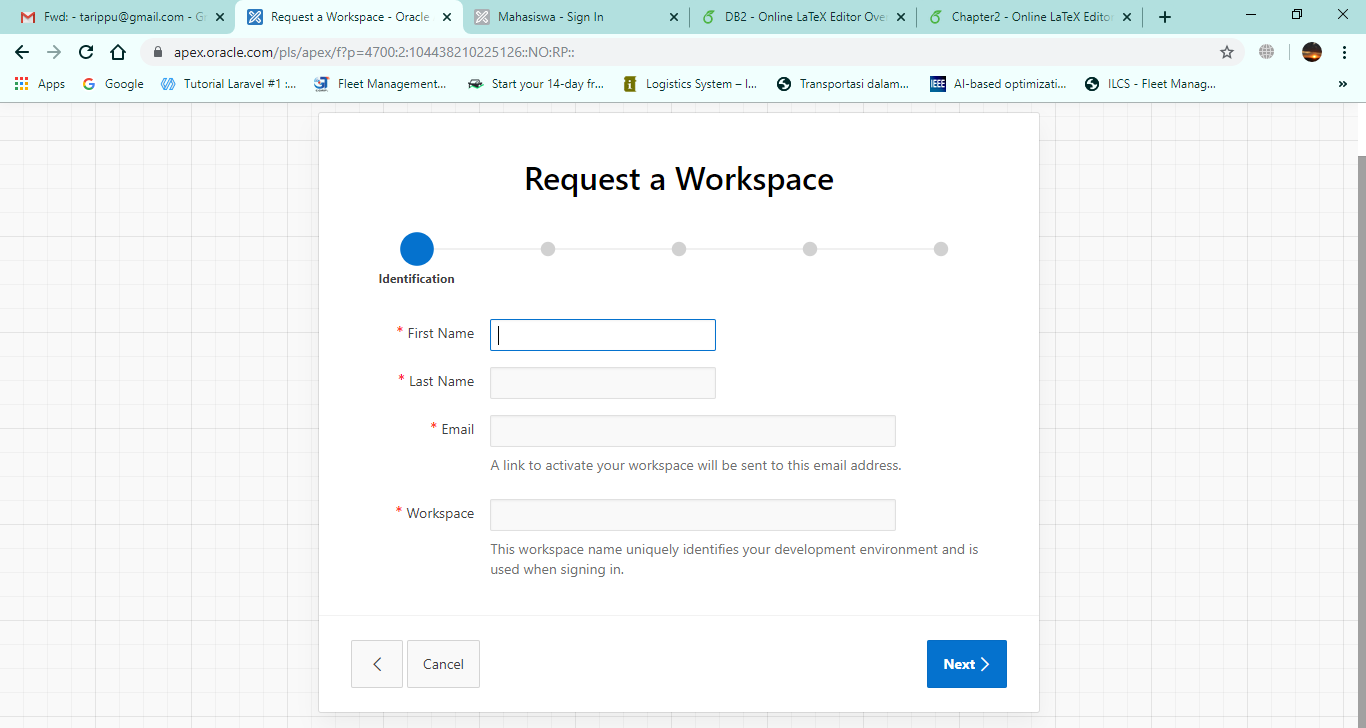
\includegraphics[width=10cm]{figures/work1.PNG}
        \caption{Workspace}
    \end{figure}
    
    \item Masukkan data-data identification yang diminta yaitu firstname, lastname, email dan nama workspace yg akan dibuat.
    \begin{figure}[!htbp]
        \centering
        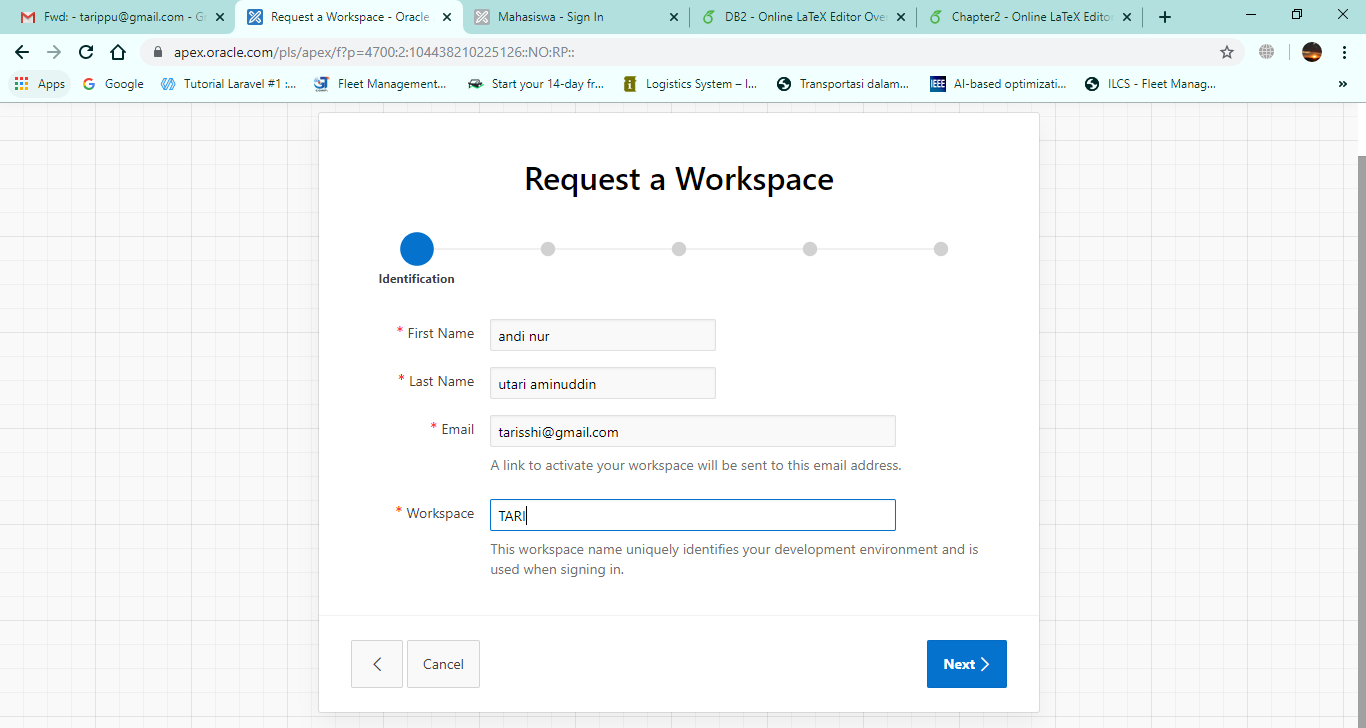
\includegraphics[width=10cm]{figures/work2.PNG}
        \caption{Identification}
    \end{figure}
    
    \newpage
    
    \item Pilih YES untuk kedua jawaban survey.
    \begin{figure}[!htbp]
        \centering
        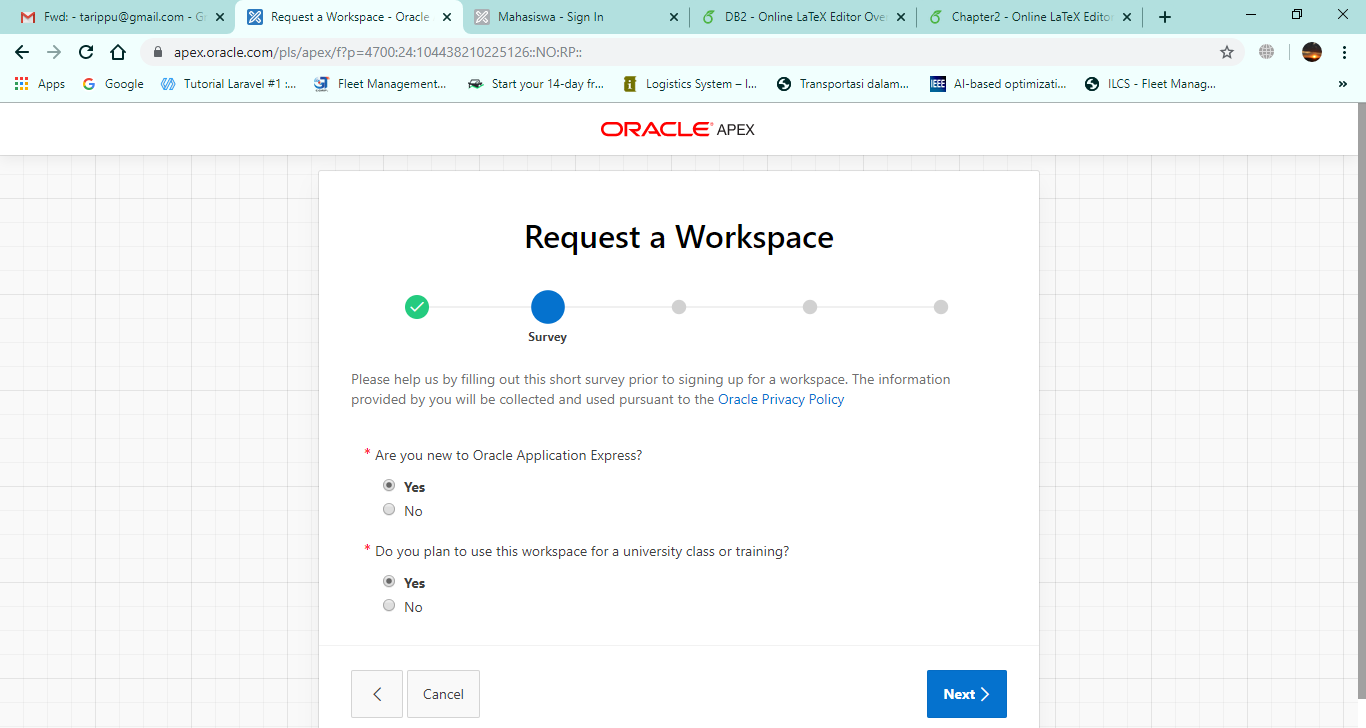
\includegraphics[width=10cm]{figures/work3.PNG}
        \caption{Survey}
    \end{figure}
    
    \item Isi Justification dengan alasan menggunakan apex.
    \begin{figure}[!htbp]
        \centering
        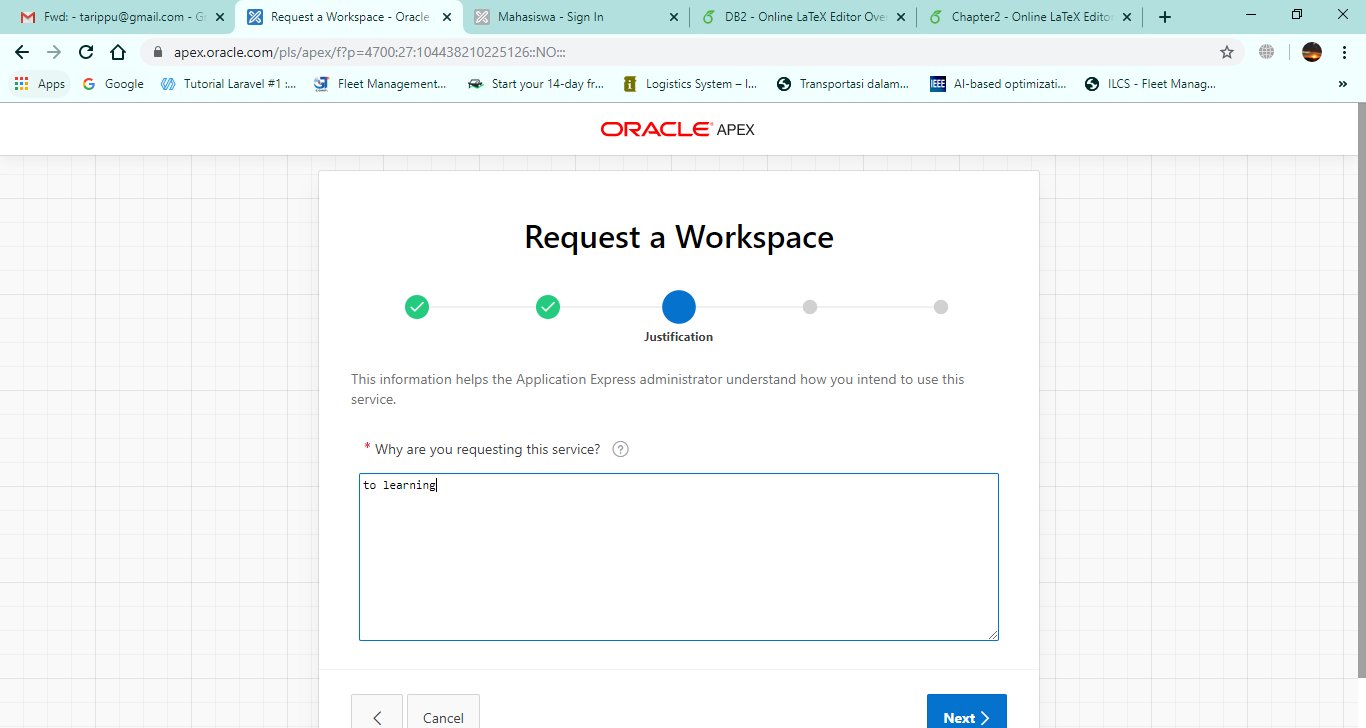
\includegraphics[width=10cm]{figures/work4.PNG}
        \caption{Justification}
    \end{figure}
    \newpage
    
    \item Klik i accept the terms untuk perintah agreement
    \begin{figure}[!htbp]
        \centering
        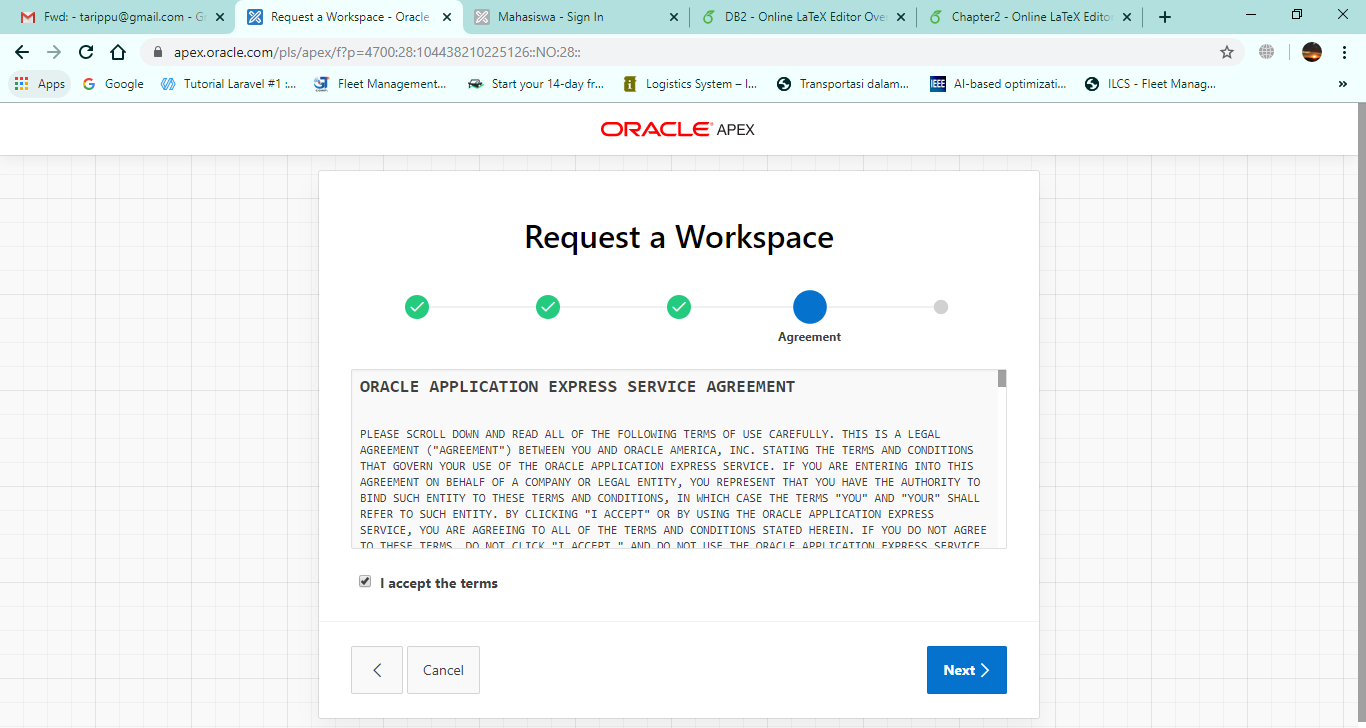
\includegraphics[width=10cm]{figures/work5.PNG}
        \caption{Agreement}
    \end{figure}
    
    \item Setelah melewati semua tahap, tahap terkahir yaitu confirmation. Klik Submit request.
    \begin{figure}[!htbp]
        \centering
        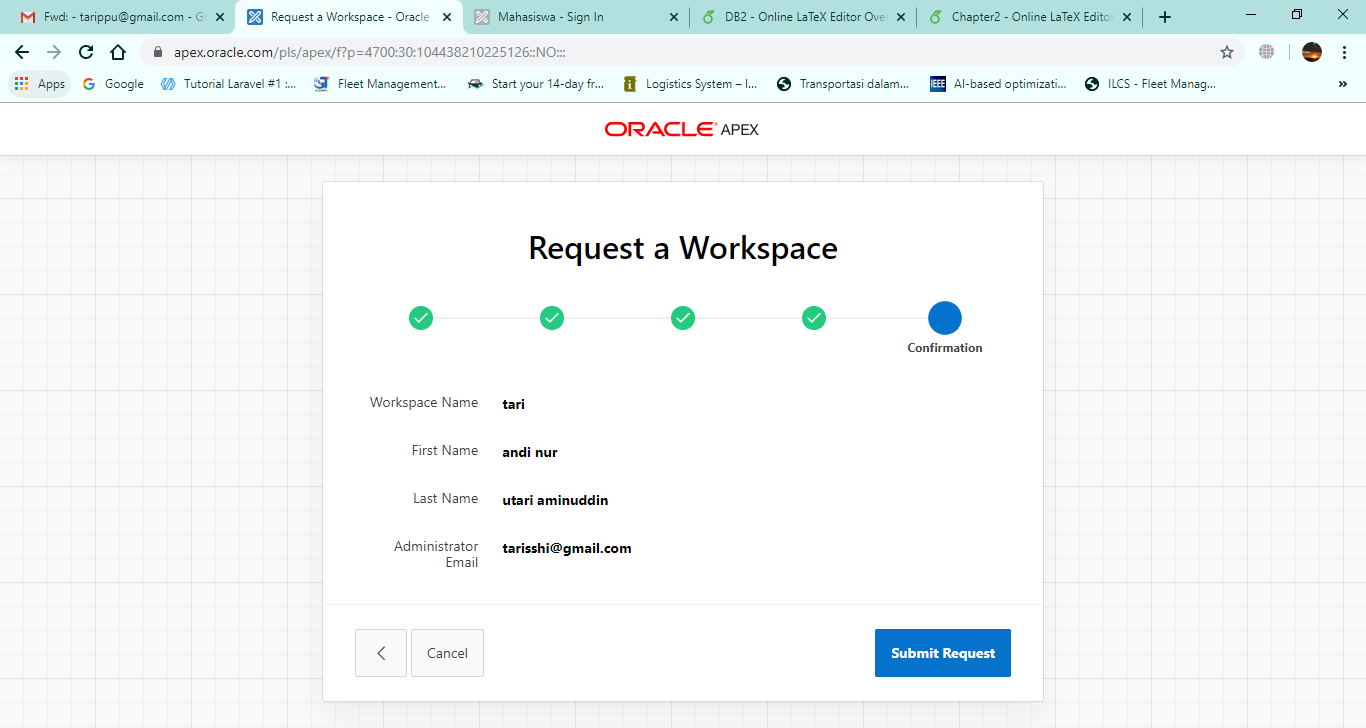
\includegraphics[width=10cm]{figures/work6.PNG}
        \caption{Buka aplikasi apex}
    \end{figure}
    
    \item buka email dan lakukan konfirmasi akun workspace dengan create workspace
    
    \newpage
    
    \item Workspace request berhasil dibuat.
    \begin{figure}[!htbp]
        \centering
        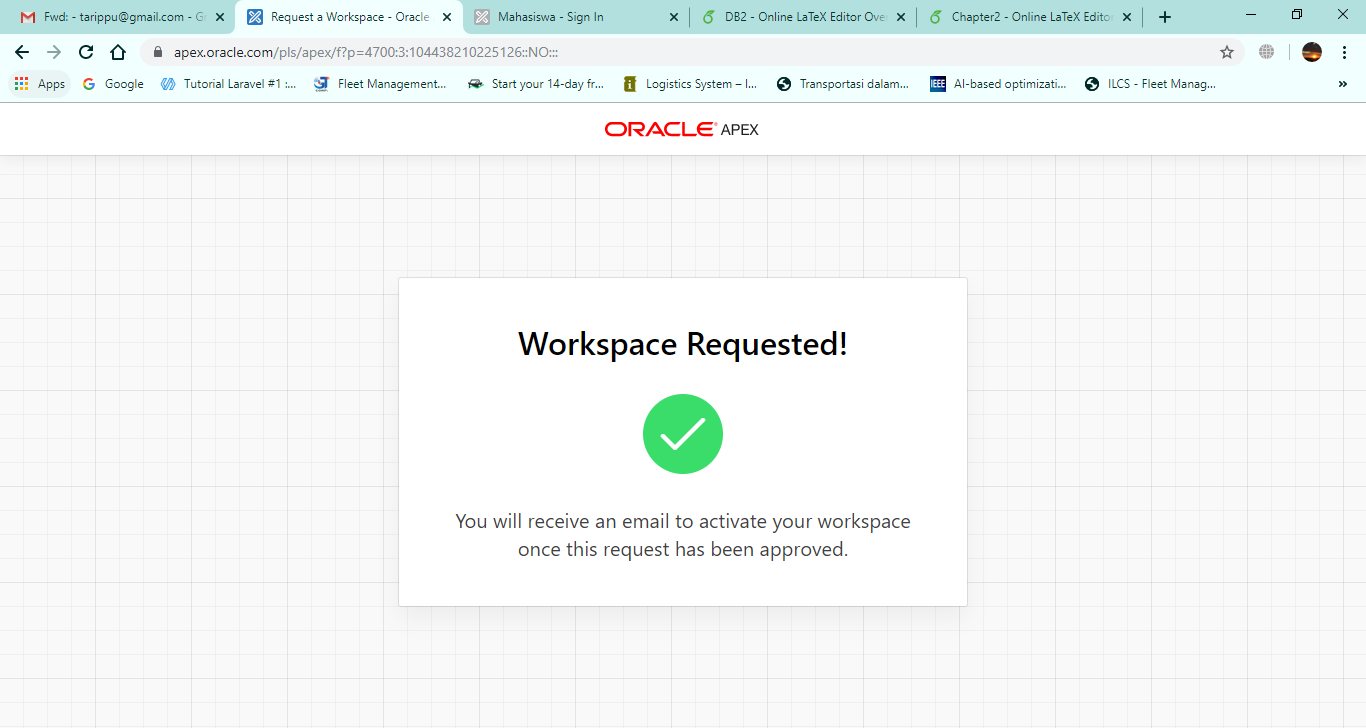
\includegraphics[width=10cm]{figures/workberhasil.PNG}
        \caption{Buka aplikasi apex}
    \end{figure}
\end{itemize}

\section{Membuat aplikasi akademik}
Berikut adalah langkah-langkah pembuatan aplikasi akademik menggunakan APEX

\begin{enumerate}
    \item Untuk membuat aplikasi akademik kita memerlukan sebuah data yang akurat dan relevan yang sudah di normalisasikan terlebih dahulu agar data tersebut tidak redudansi untuk meminimalisir penggunaan data yang berulang. data yang akan digunakan yaitu data mahasiswa sebagai berikut:
    \begin{figure}[!htbp]
        \centering
        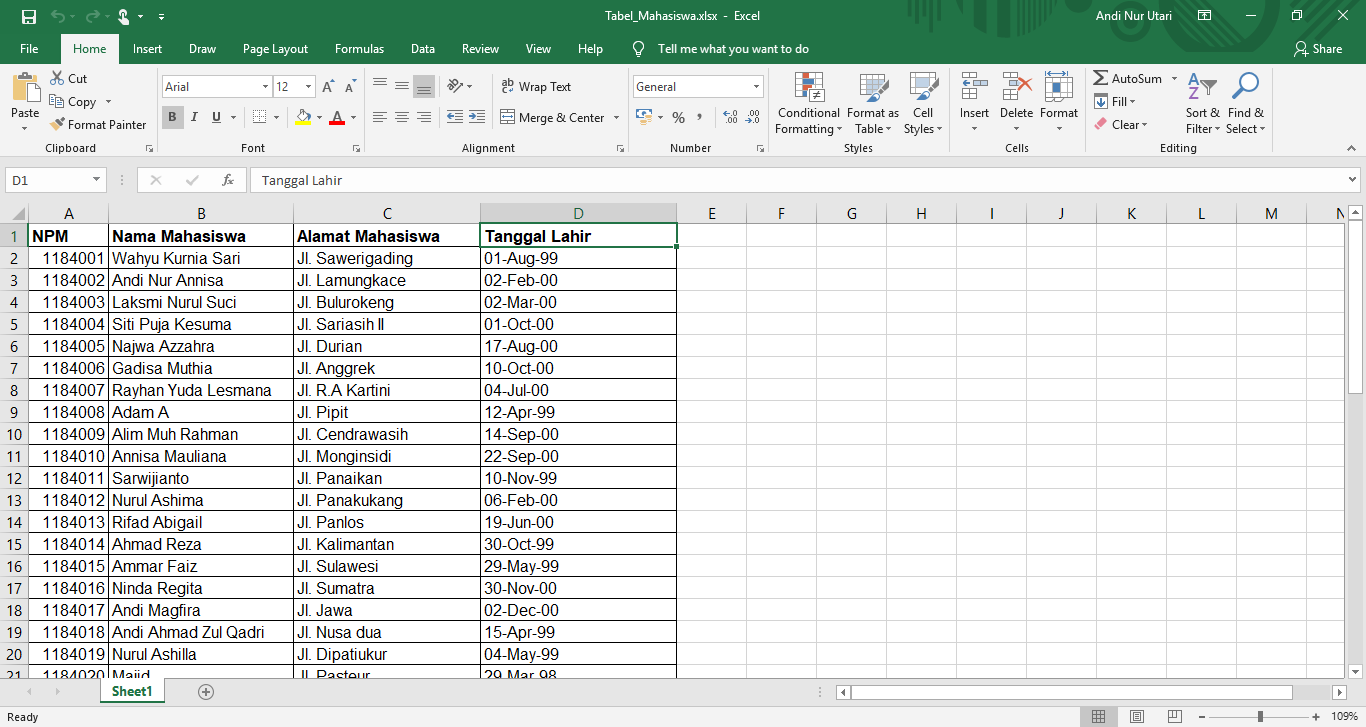
\includegraphics[width=15cm]{figures/01.PNG}
        \caption{Tabel Mahasiswa}
    \end{figure}
    
    \item Buat File tabel baru untuk memisahkan data-data dari tabel mahasiswa menjadi beberapa tabel lalu diberikan kode pada setiap tabel untuk dijadikan primary key.

    
    \item Buka aplikasi oracle apex online atau link berikut\\ https://apex.oracle.com/pls/apex/f?p=4550:1:16642045919295:::::

    \item Login dengan memasukkan workspace, username, dan password yang sudah dibuat.
    \begin{figure}[!htbp]
        \centering
        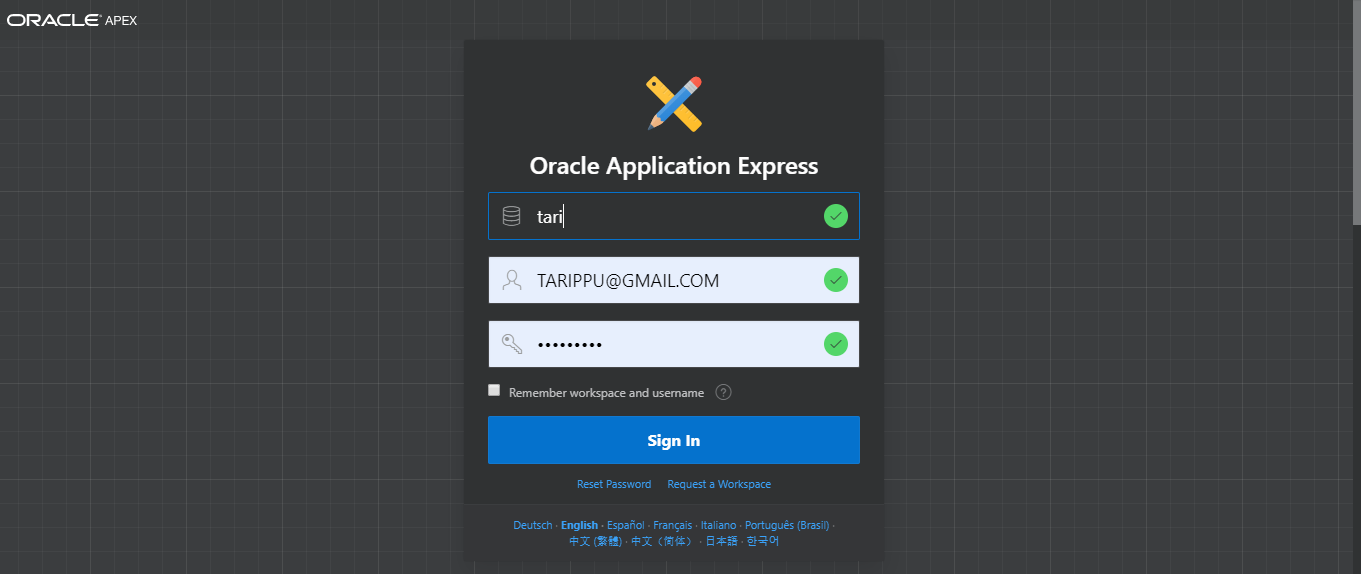
\includegraphics[width=13cm]{figures/login.PNG}
        \caption{Login}
    \end{figure}
    
    {Account APEX}
    \begin{itemize}
        \item WORKSPACE : tari
        \item USERNAME  : tarippu@gmail.com
        \item PASS      : taritari2
    \end{itemize}
    \newpage
    
    \item Setelah berhasil login akan muncul tampilan utama apex oracle, lalu klik sql workshop drop down pilih utilities lalu drop down pilih data workshop
    \begin{figure}[!htbp]
        \centering
        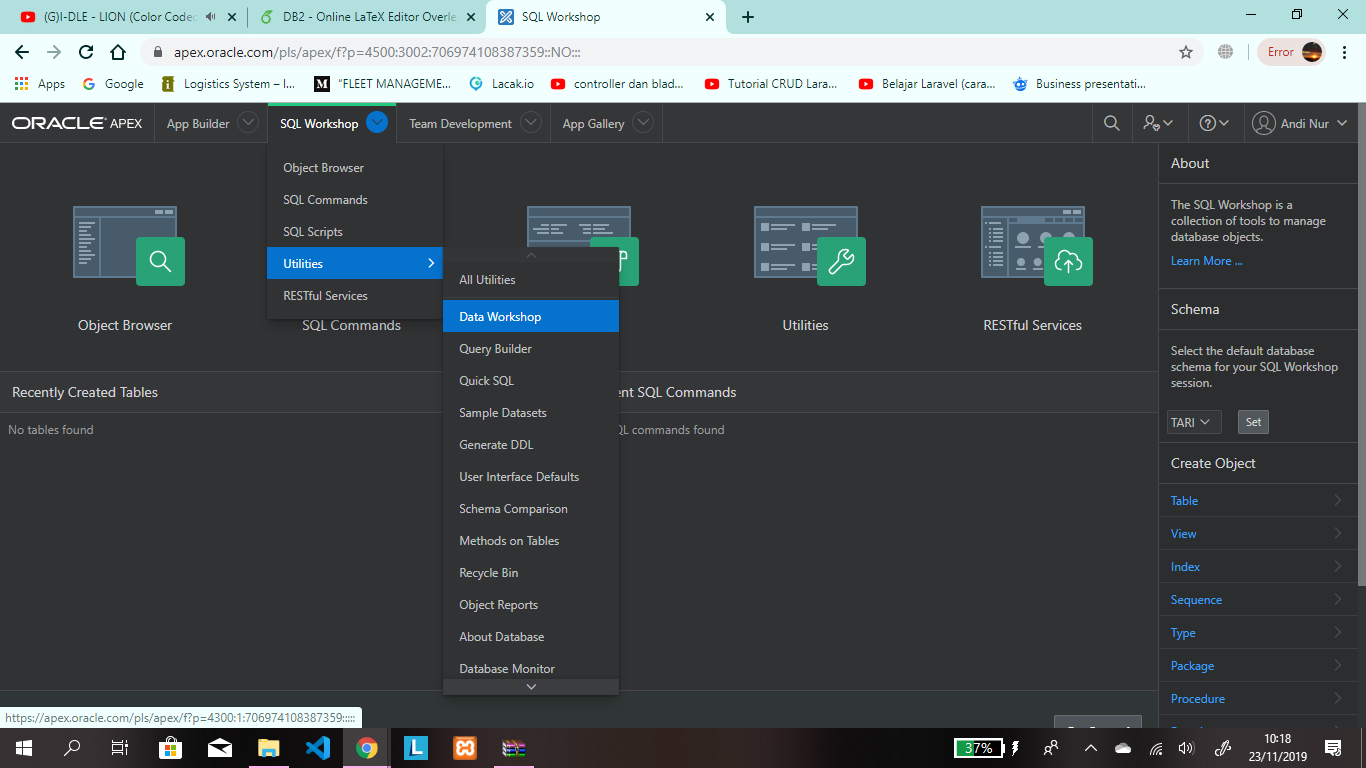
\includegraphics[width=13cm]{figures/Screenshot(9).png}
        \caption{Data Workshop}
    \end{figure}
     
    \item Lalu klik load data, upload file/data pilih data yang ingin ditambahkan
    \begin{figure}[!htbp]
        \centering
        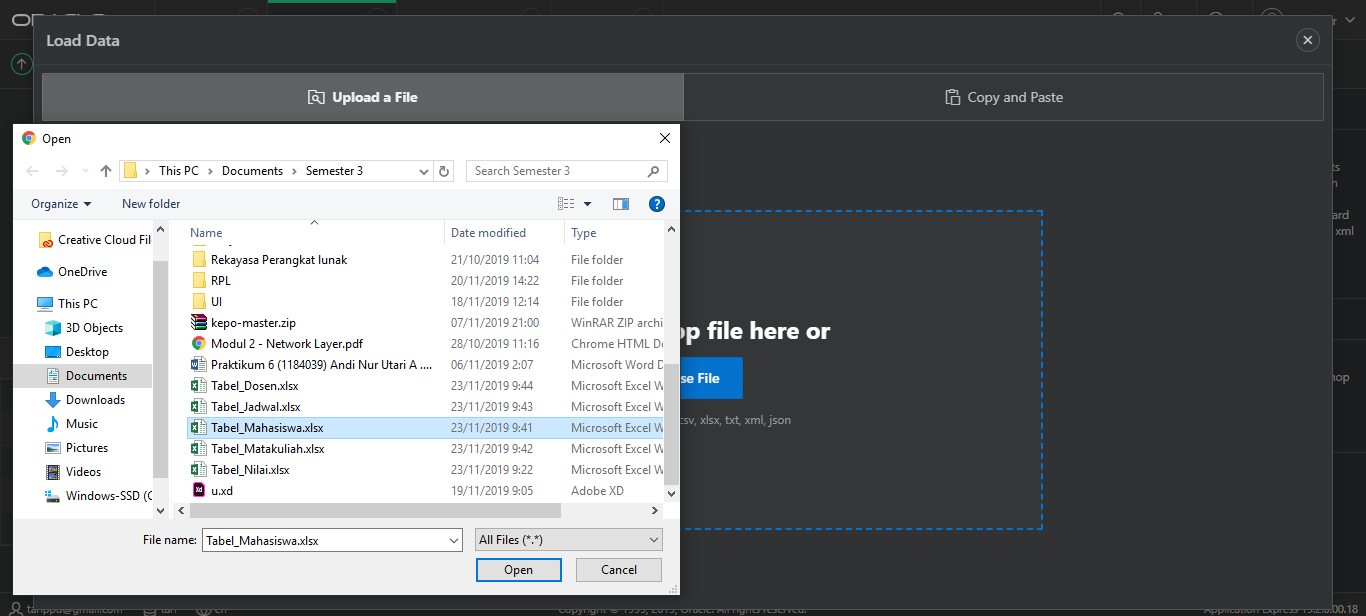
\includegraphics[width=13cm]{figures/1.PNG}
        \caption{Create}
    \end{figure}
   
    \item Masukkan semua data tabel yang sudah dipisahkan tadi lalu berikan nama table sesuai namanya.
    \newpage 
    
    \item Isi table name, dengan nama MAHASISWA. lalu klik secara otomatis error table namenya akan terisi.
    \begin{figure}[!htbp]
        \centering
        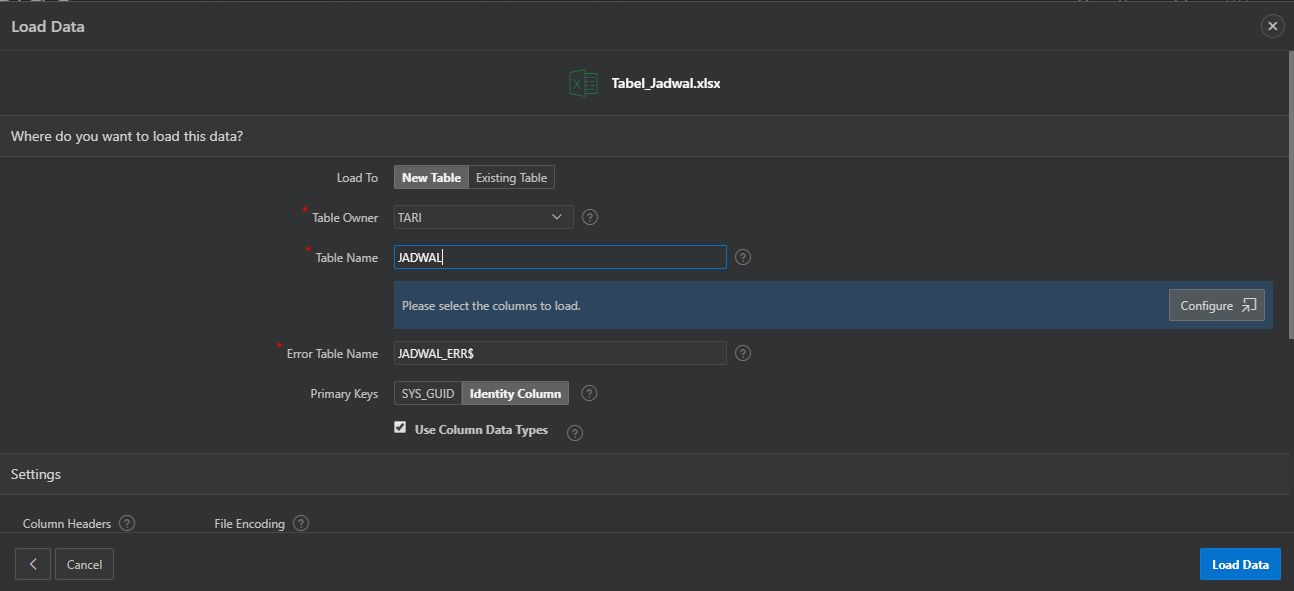
\includegraphics[width=13cm]{figures/namedata.PNG}
        \caption{Isi Nama}
    \end{figure}

    \item klik configure disebelah kanan. Lalu akan ditampilkan isi dari data/table yang di tambahkan klik save changes
    \begin{figure}[!htbp]
        \centering
        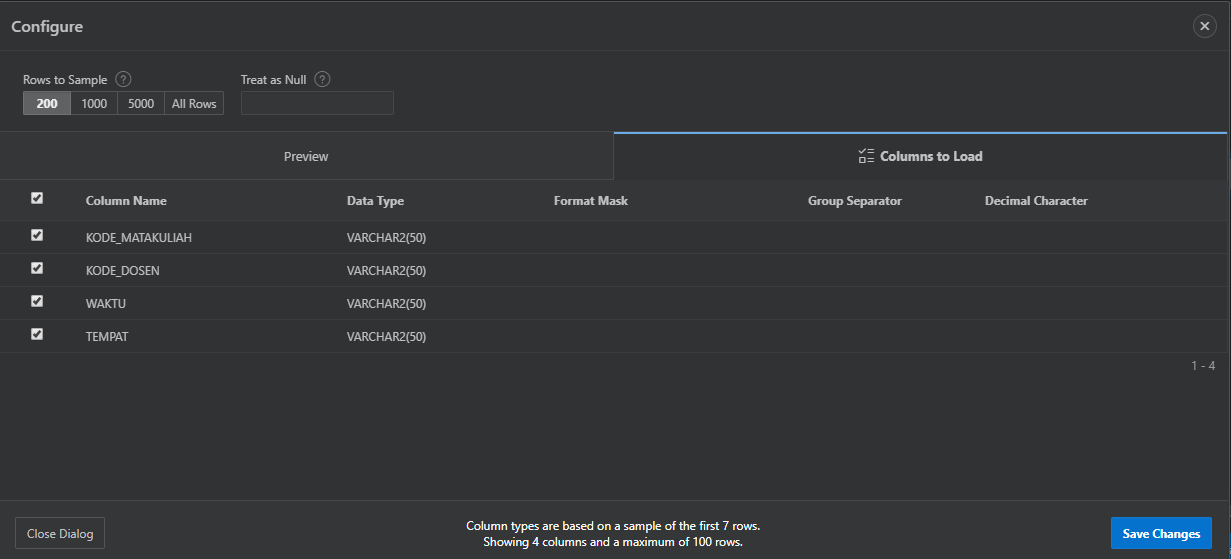
\includegraphics[width=13cm]{figures/2.PNG}
        \caption{Congifure}
    \end{figure}
    
    \newpage
    \item Setelah muncul isi data dan tidak ada yang error dan congfiurasi berhasil. Klik load data Maka akan muncul jumlah rows pada table yg sudah di created. 
    \begin{figure}[!htbp]
        \centering
        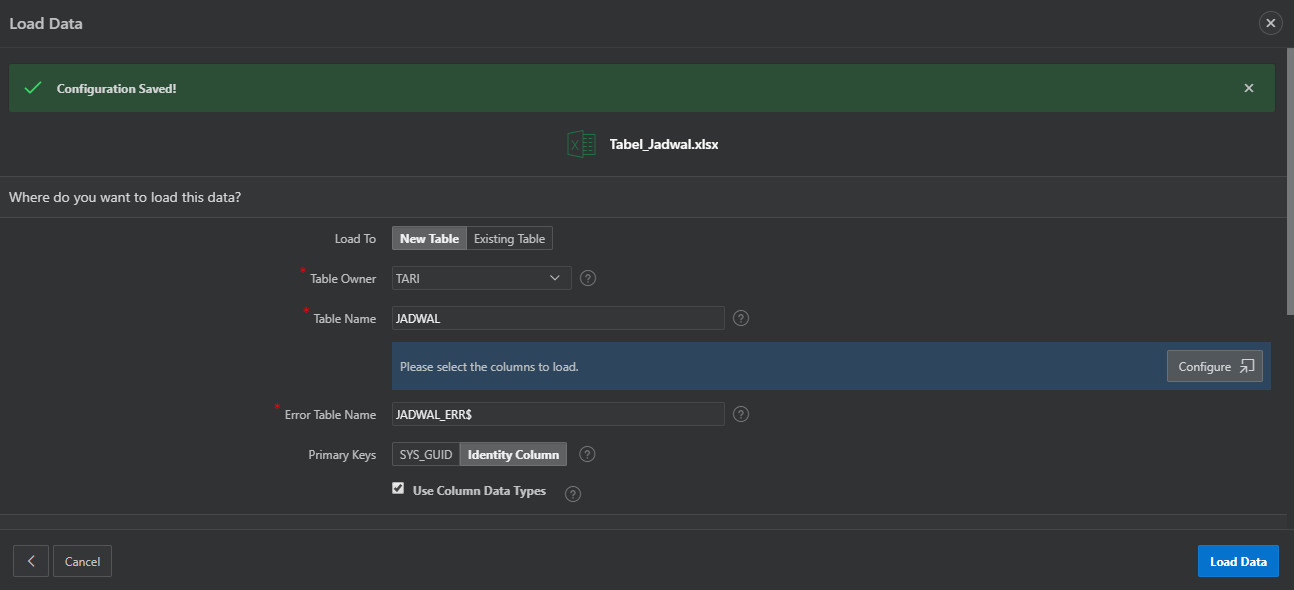
\includegraphics[width=13cm]{figures/3.PNG}
        \caption{Load Data}
    \end{figure}

    \item Untuk Melihat semua table yang sudah di crate dapat dilihat pada objek browser di SQL Workshop
    \begin{figure}[!htbp]
        \centering
        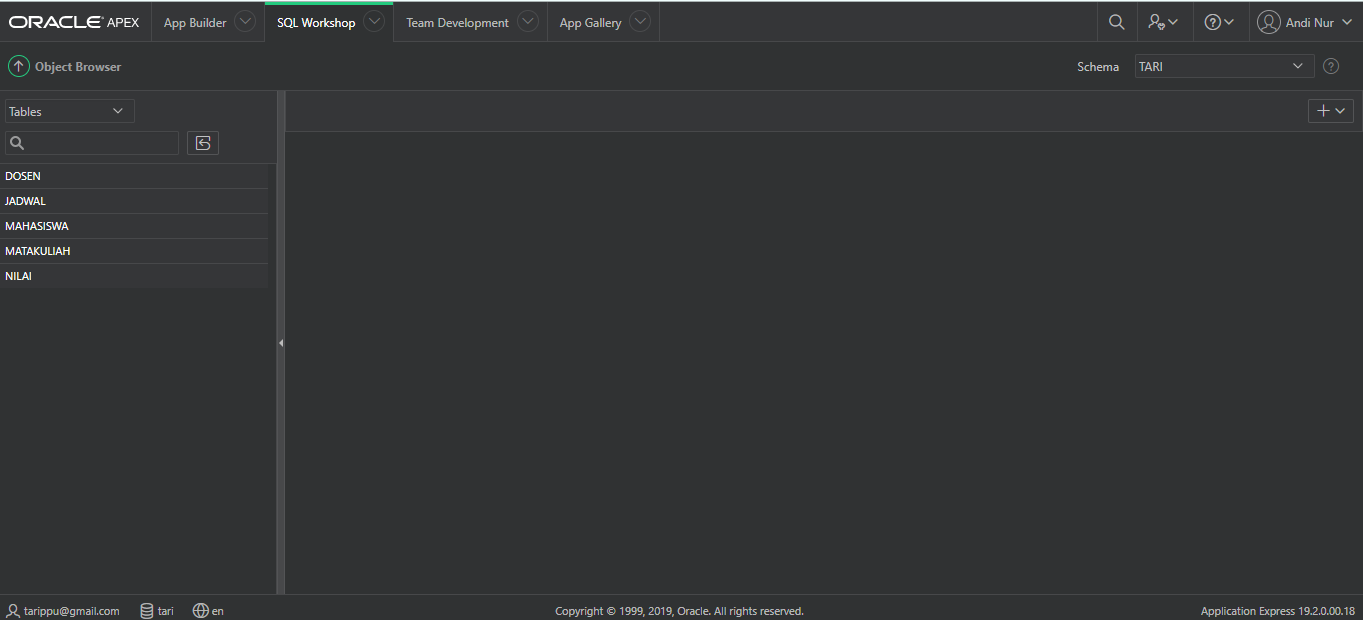
\includegraphics[width=13cm]{figures/4.PNG}
        \caption{Objek browser list data}
    \end{figure}
    \newpage
    
    \item Hapus ID pada semua table yang sudah dibuat, buka SQL command lalu ketikkan perintah untuk menhapus ID pada masing-masing data.
        \begin{figure}[!htbp]
        \centering
        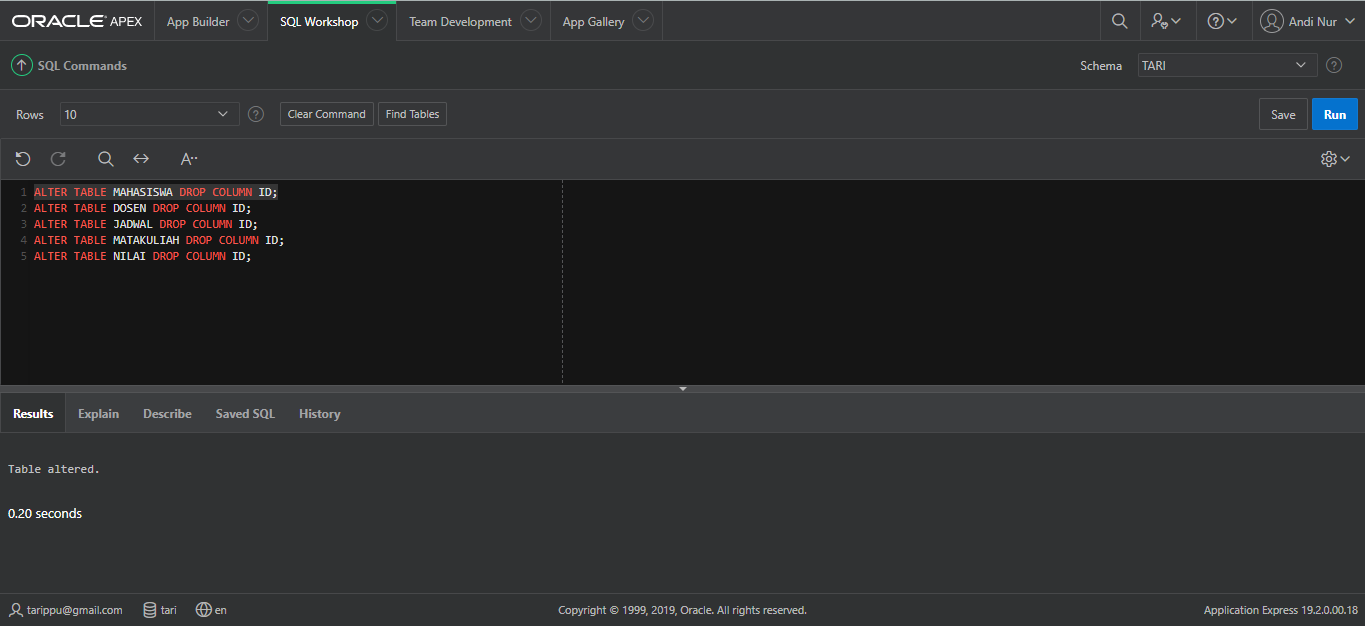
\includegraphics[width=13cm]{figures/5.PNG}
        \caption{Hapus ID}
    \end{figure}
    
    Berikut perintahnya, untuk menjalankan nya blok satu-satu lalu klik run.
    \begin{verbatim}
        ALTER TABLE MAHASISWA DROP COLUMN ID;
        ALTER TABLE DOSEN DROP COLUMN ID;
        ALTER TABLE JADWAL DROP COLUMN ID;
        ALTER TABLE MATAKULIAH DROP COLUMN ID;
        ALTER TABLE NILAI DROP COLUMN ID;
    \end{verbatim}
    
    \item Tambahkan foreign key dan primary key pada setiap table pada SQL command.untuk menjalankan perintah sql command kita harus block kode yg akan dijalankan lalu klik run.
     \begin{verbatim}
        ALTER TABLE MAHASIWA
        ADD PRIMARY KEY (NPM);
        ALTER TABLE DOSEN
        ADD PRIMARY KEY (KODE_DOSEN);
        ALTER TABLE MATAKULIAH 
        ADD PRIMARY KEY (KODE_MATAKULIAH);
    \end{verbatim}
    \newpage
        \begin{figure}[!htbp]
        \centering
        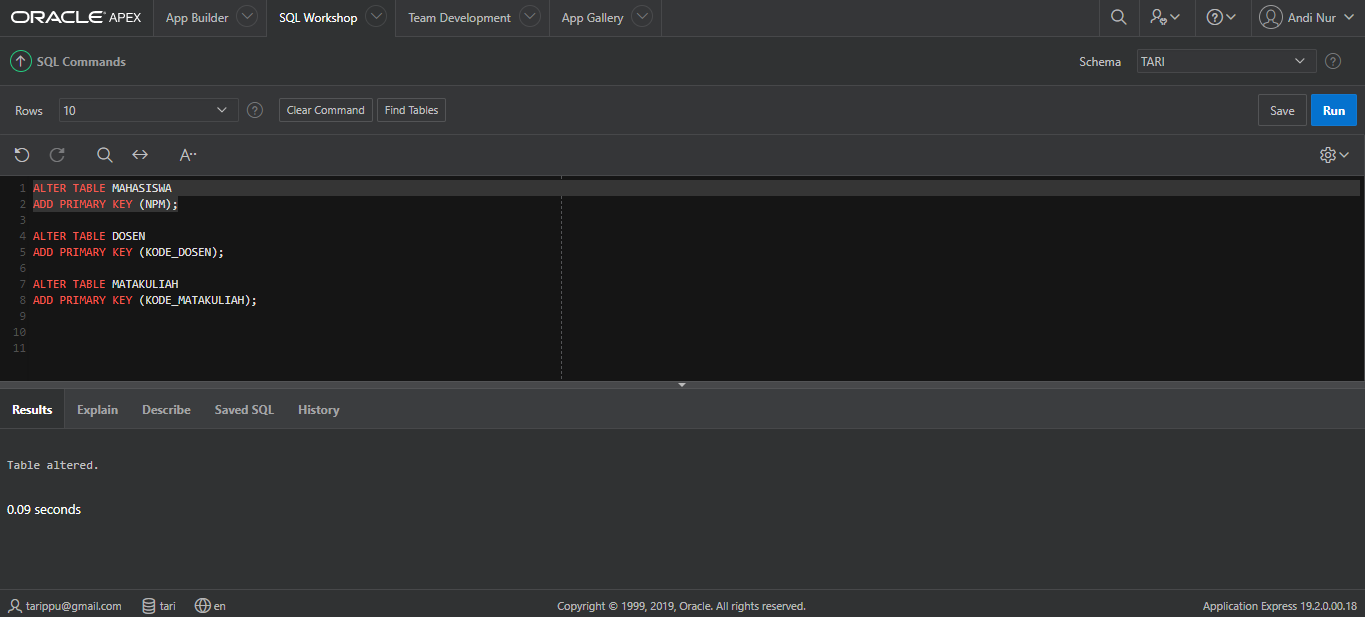
\includegraphics[width=13cm]{figures/6.PNG}
        \caption{Add Primary Key}
    \end{figure}    
    
     \item Berikut kodingan pada SQL Command untuk menabahkan foreign key dari tabel lainnya untuk menjalankan perintah sql command kita harus block kode yg akan dijalankan lalu klik run.
        \begin{verbatim}
        ALTER TABLE JADWAL
        ADD FOREIGN KEY (KODE_MATAKULIAH)
        REFERENCES MATAKULIAH (KODE_MATAKULIAH);

        ALTER TABLE JADWAL
        ADD FOREIGN KEY (KODE_DOSEN)
        REFERENCES DOSEN (KODE_DOSEN);

        ALTER TABLE NILAI
        ADD FOREIGN KEY (NPM)
        REFERENCES MAHASISWA (NPM);

        ALTER TABLE JADWAL
        ADD FOREIGN KEY (KODE_MATAKULIAH)
        REFERENCES MATAKULIAH (KODE_MATAKULIAH);
    \end{verbatim}
    \newpage
        \begin{figure}[!htbp]
        \centering
        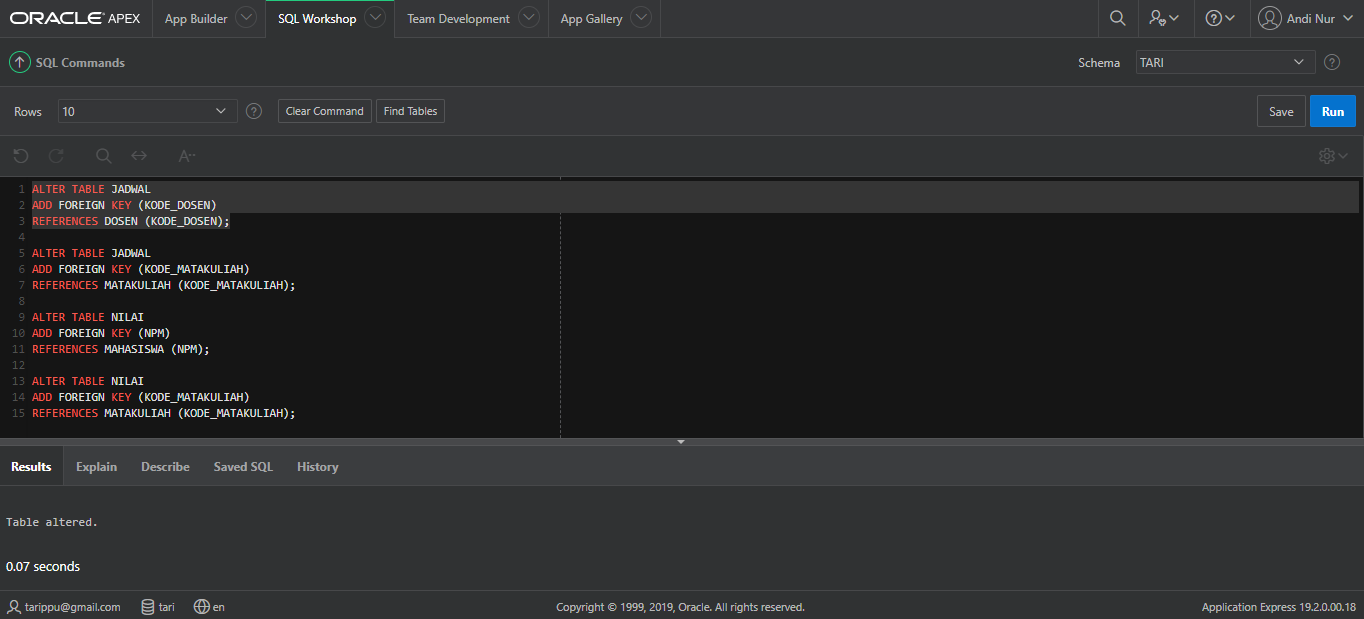
\includegraphics[width=13cm]{figures/7.PNG}
        \caption{Add Foreign Key}
    \end{figure}  

     \item Untuk menambahkan table, menghapus atau ingin mengubah data yg sudah ada dapat di lakukan pada SQL Commands. 

    \item Pilih menu app builder lalu create, pilih new application.
    \begin{figure}[!htbp]
        \centering
        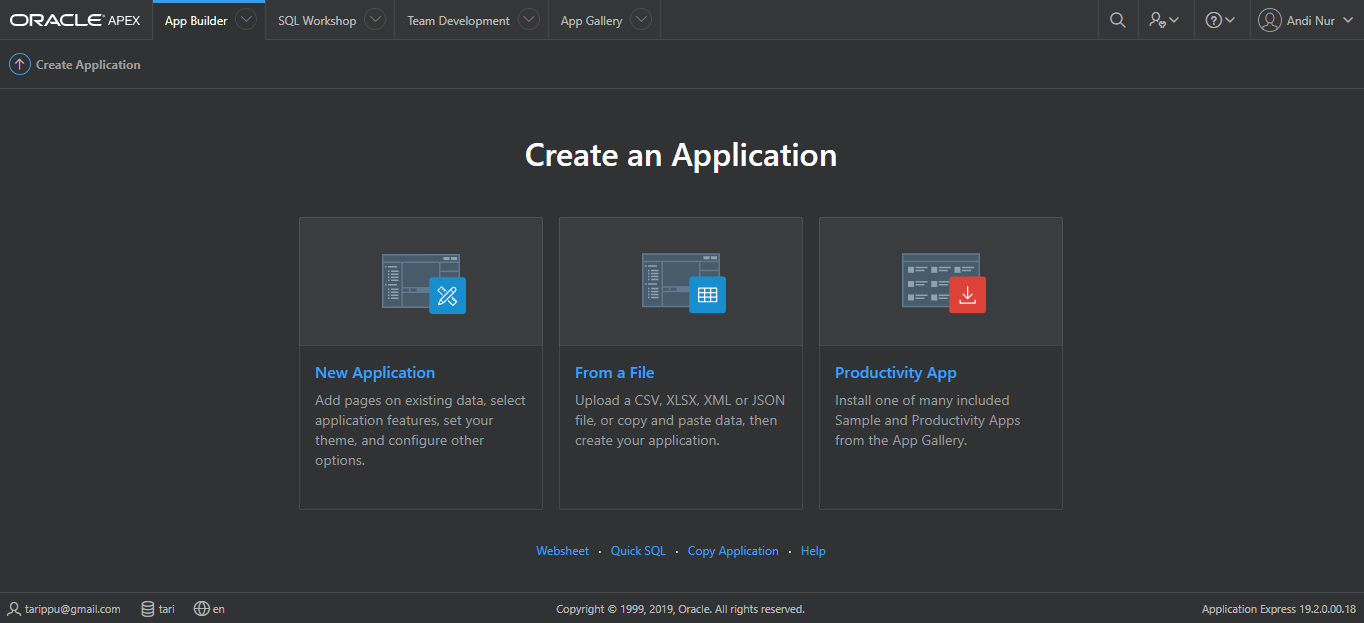
\includegraphics[width=13cm]{figures/8.PNG}
        \caption{Create new application}
    \end{figure} 
    
    \newpage
    \item Tambahkan nama aplikasi yang ingin dibuat 
        \begin{figure}[!htbp]
        \centering
        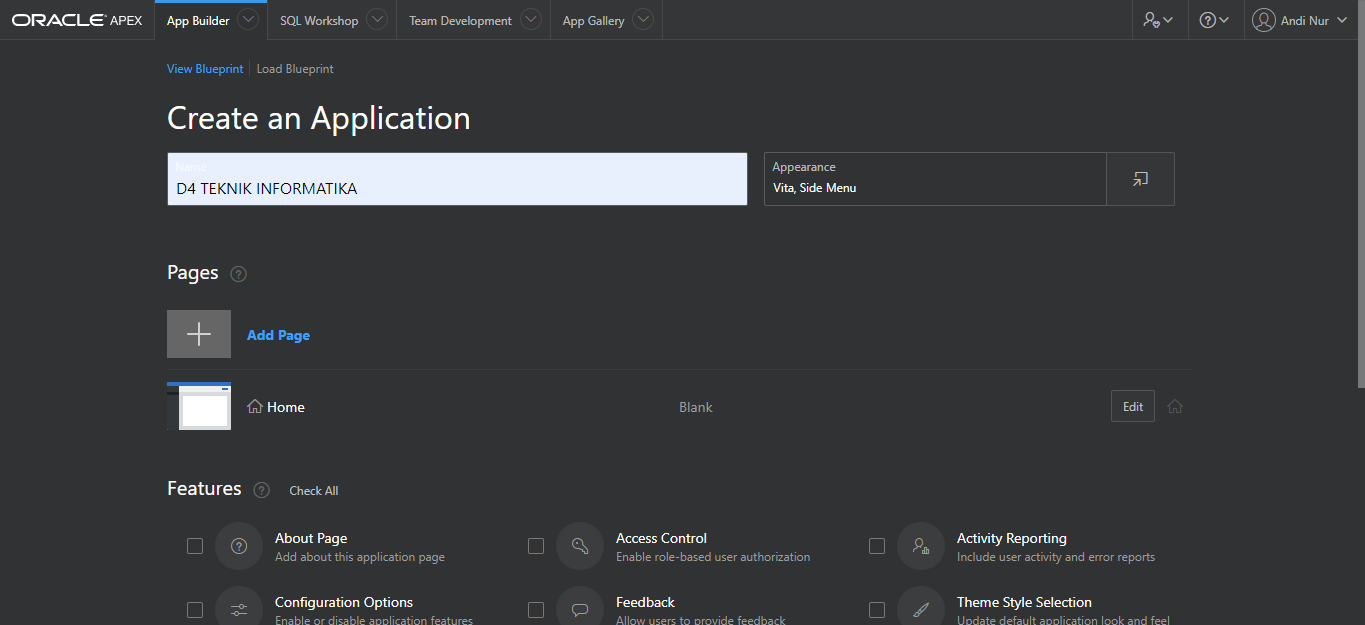
\includegraphics[width=13cm]{figures/nameapp.PNG}
        \caption{Tambahkan nama aplikasi}
    \end{figure}
    
    \item Klik add page lalu pilih interactive report
        \begin{figure}[!htbp]
        \centering
        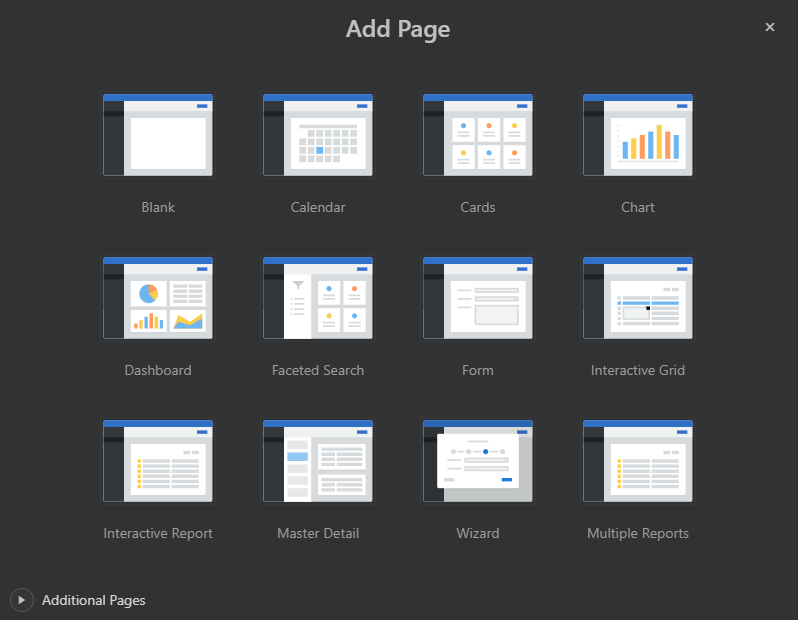
\includegraphics[width=13cm]{figures/10.PNG}
        \caption{Add page interaktive report}
    \end{figure}
    
    \newpage
    \item Isi page name (mahasiswa) dan pilih tabel yang sesuai dengan mengklik ikon disebelah kanan pada tabel or view lalu pilih tabel nya. Lakukan hal yang sama untuk Matakuliah dan Dosen. Kemudian klik add page.
        \begin{figure}[!htbp]
        \centering
        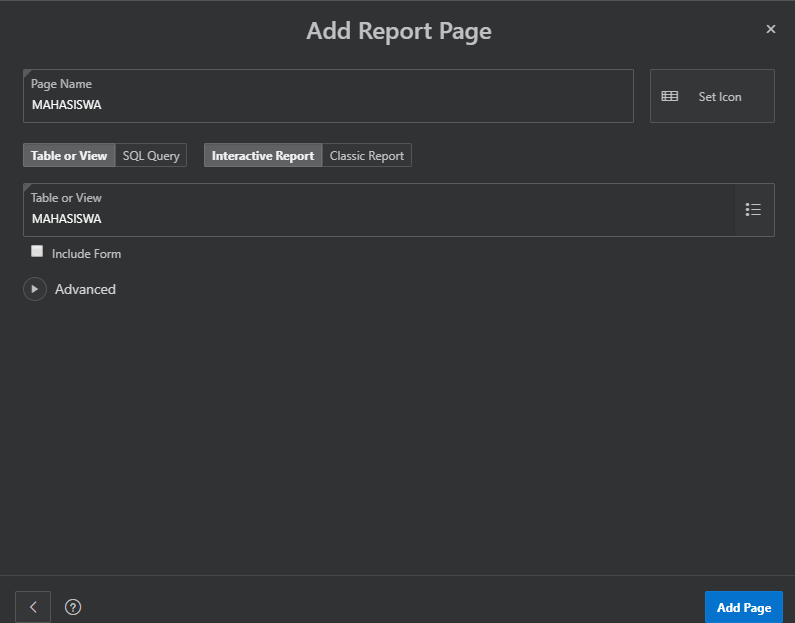
\includegraphics[width=9cm]{figures/18.PNG}
        \caption{Add report page Mahasiswa, Dosen dan Matakuliah}
    \end{figure}
    
    \item Untuk menambahkan data Jadwal lakukan seperti hal diatas namun yang membedakan yaitu tidak dengan table or view melainkan klik SQL query dan tambahkan perintah inner join pada SQL query seperti dibawah ini. Kemudian klik add page.
        \begin{figure}[!htbp]
        \centering
        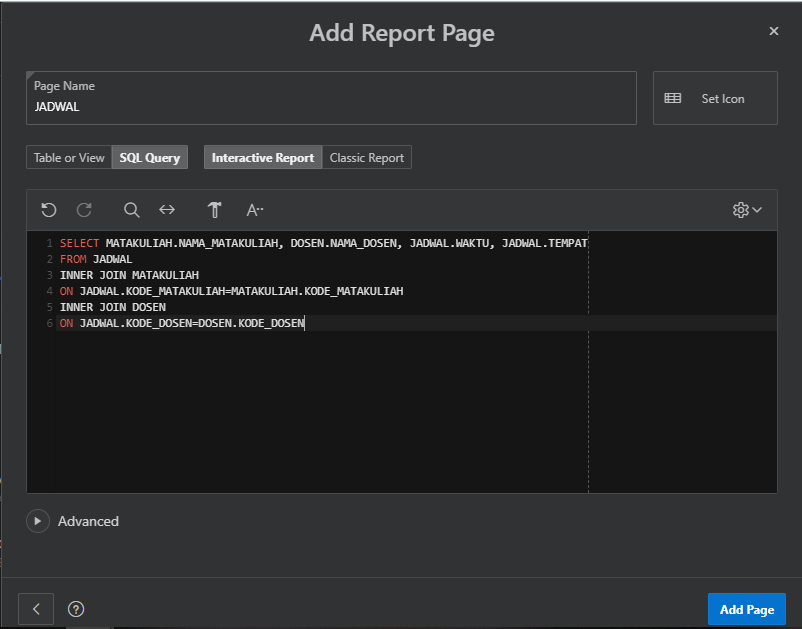
\includegraphics[width=9cm]{figures/11.PNG}
        \caption{Add report page Jadwal}
    \end{figure}
    
    \item Terakhir untuk menambahkan data Nilai sama dengan cara menambahkan data Jadwal yaitu tidak dengan table or view melainkan klik SQL query dan tambahkan perintah inner join pada SQL query seperti dibawah ini. Kemudian klik add page.
        \begin{figure}[!htbp]
        \centering
        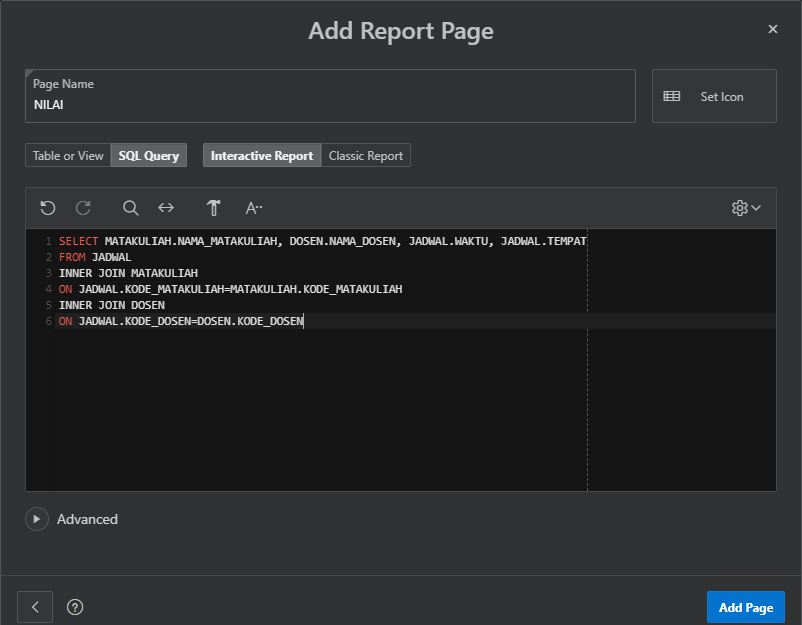
\includegraphics[width=10cm]{figures/12.PNG}
        \caption{Add report page Nilai}
    \end{figure}
    
    \item Setelah semua data sudah di tambahkan seperti berikut, lalu klik create application.
        \begin{figure}[!htbp]
        \centering
        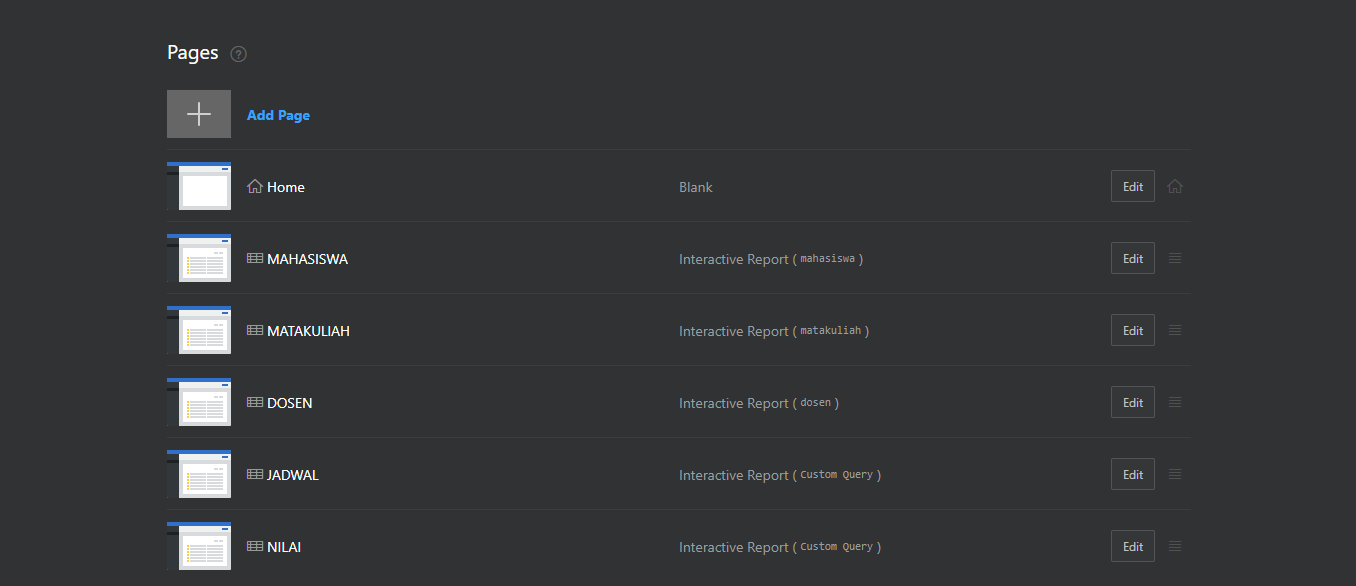
\includegraphics[width=13cm]{figures/14.PNG}
        \caption{Create Aplication}
    \end{figure}
    
    \newpage
    \item Selanjutnya akan menuju ke menu App builder lalu klik run application untuk menjalankan aplikasi yang sudah dibuat.
        \begin{figure}[!htbp]
        \centering
        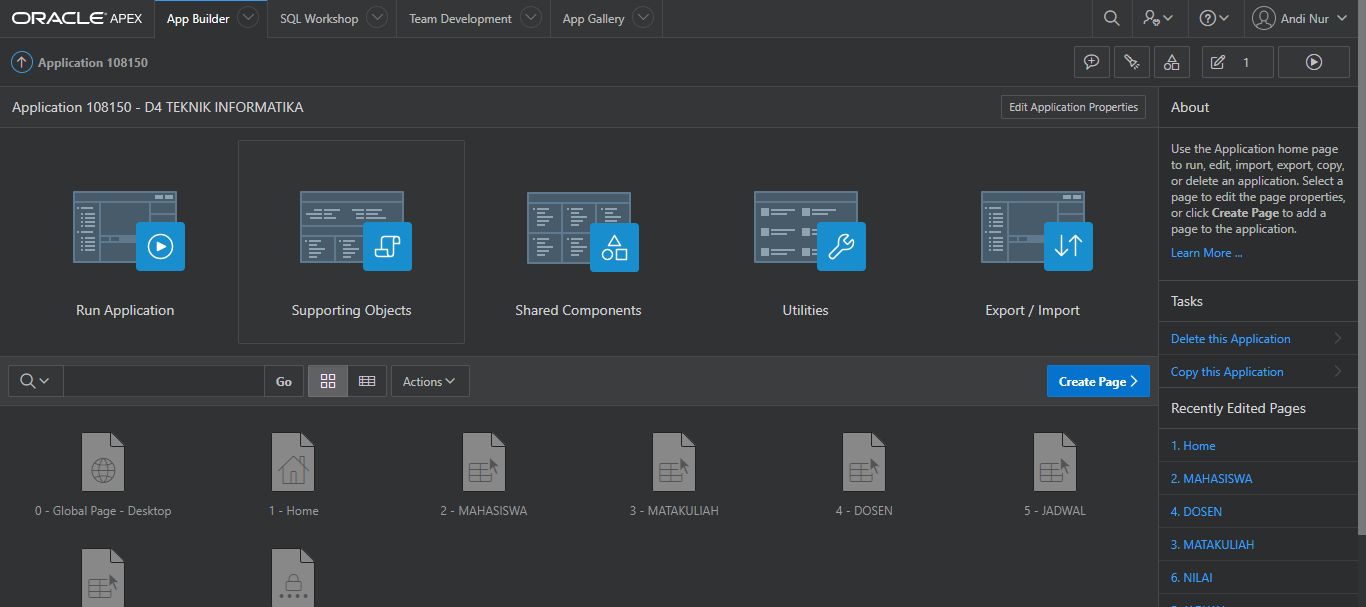
\includegraphics[width=13cm]{figures/15.PNG}
        \caption{Run Application}
    \end{figure}
    
    \item Sebelum masuk ke aplikasi kita harus melewati tahapan login. masukkan username/email dan password nya.\\
    \textbf{Username : tarippu@gmail.com}\\
    \textbf{Password : taritari2}
        \begin{figure}[!htbp]
        \centering
        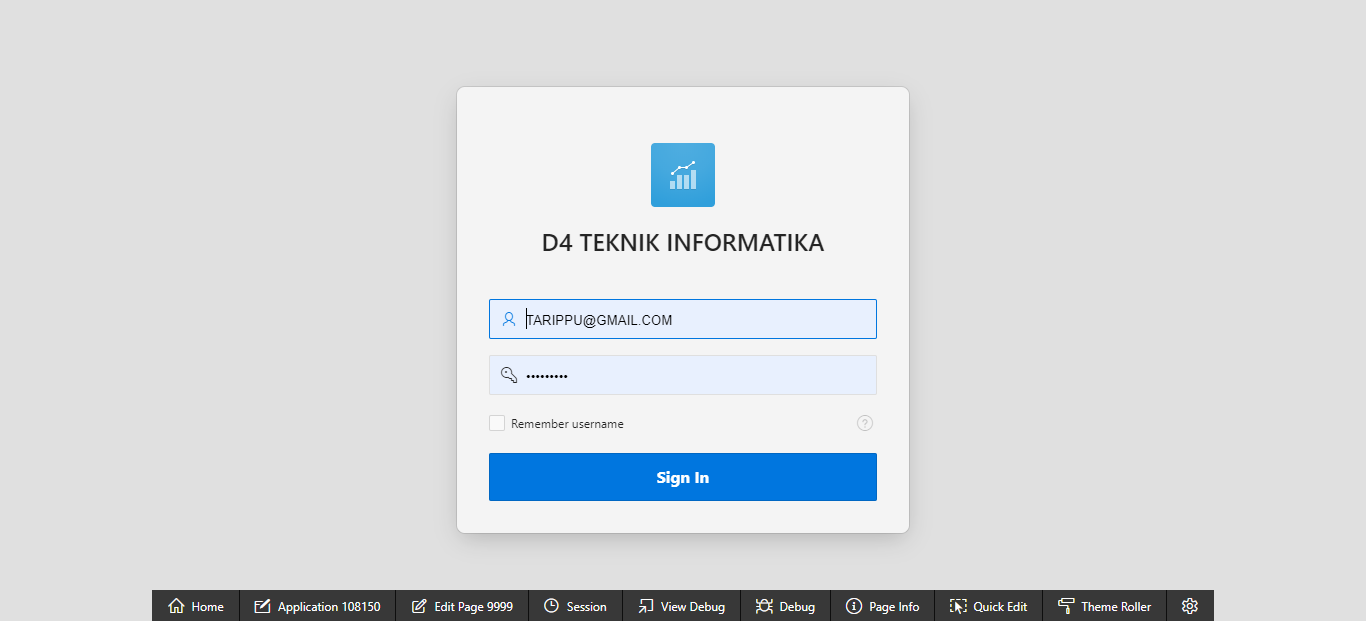
\includegraphics[width=13cm]{figures/16.PNG}
        \caption{Login Aplikasi D4 TEKNIK INFORMATIKA}
    \end{figure}    
    
    \newpage
    
    \item Setelah login dan masuk ke aplikasi yang pertama kali di tampilan dari Aplikasi D4 TEKNIK INFORMATIKA yang sudah dibuat tadi yaitu menu utama, lalu ada menu Mahasiswa, Dosen, Jadwal, Matakuliah dan Nilai.
        \begin{figure}[!htbp]
        \centering
        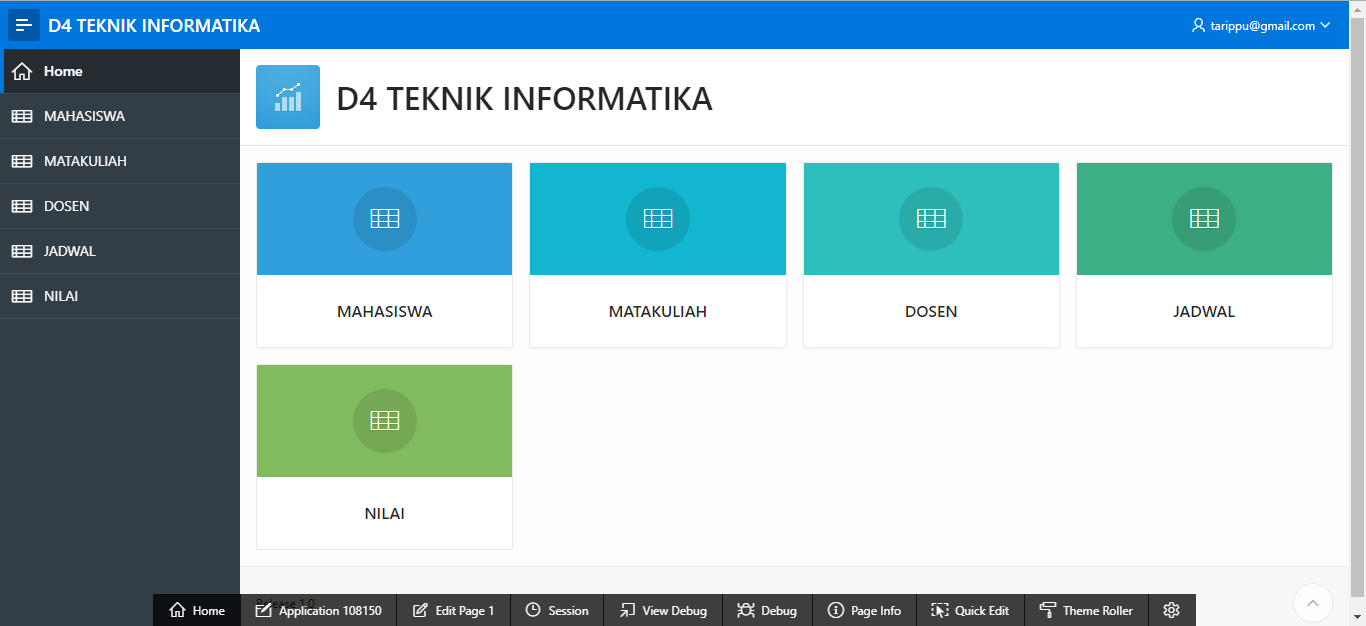
\includegraphics[width=13cm]{figures/17.PNG}
        \caption{Aplikasi D4 TEKNIK INFORMATIKA}
    \end{figure}
\end{enumerate}
